% Slide-n
\begin{frame}[t]{Distribution}
	\begin{figure}[h]
		\centering
		\begin{subfigure}{0.45\textwidth}
			\centering
			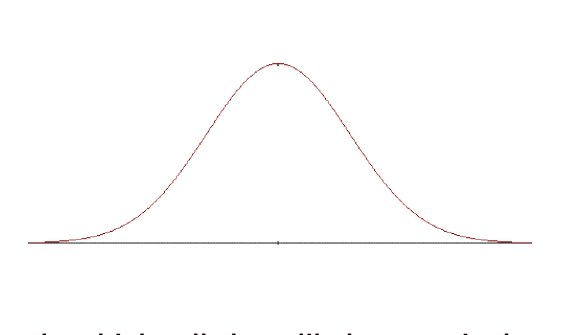
\includegraphics[trim={0 1cm 0 0}, clip, scale=0.4]{eda/nd.png}
			\caption{Values close to the mean are more likely}
		\end{subfigure}
		\hfil
		\begin{subfigure}{0.45\textwidth}
			\centering
			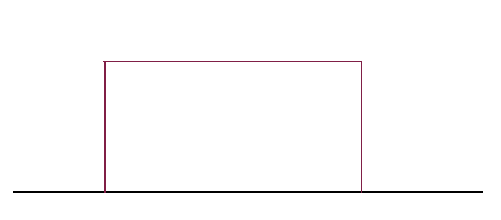
\includegraphics[scale=0.5]{eda/nd2.png}
			\caption{All values are equally likely}
		\end{subfigure}
		
	\end{figure}
\end{frame}

\begin{frame}[t]{The Normal Curve}
	\begin{itemize}
		\item The distributions of most continuous random variables will follow 
		the shape of the normal curve.
		\item Mean, Median and Mode all exist at the center.
		
	\end{itemize}
\begin{figure} [ht]
	\centering
	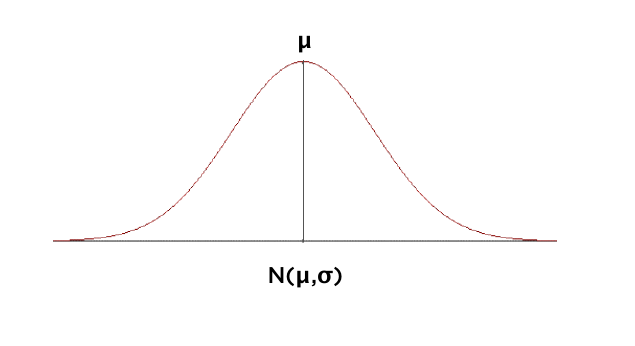
\includegraphics[trim={0 1cm 0 0}, clip, scale=0.4]{eda/nd3.png}
\end{figure}
\centering
A formula which tells how likely a particular value is
to occur in your data.
\end{frame}
% Slide-n
\begin{frame}[t]{The Empirical Rule--1}
	The empirical rule tells you what percentage of your data falls within a 
	certain number of standard deviations from the mean.
	\begin{itemize}
		\item 68\% of all values fall within 1 standard deviation of the mean.
		\item 95\% of the all values fall within 2 standard deviation of the 
		mean. 
		\item 99.7\% of the all values fall within 3 standard deviation of the 
		mean. 
	\end{itemize}

\begin{figure} [ht]
	\centering
	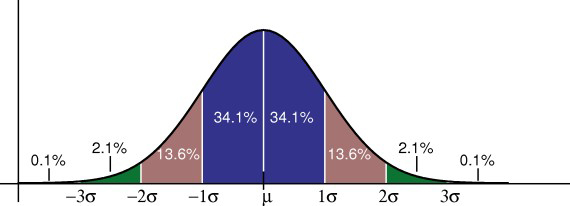
\includegraphics[width=0.5\textwidth]{eda/standard-normal-distribution.jpg}
	\source{\url{https://www.statisticshowto.com/probability-and-statistics/normal-distributions/}}
\end{figure}
\end{frame}


\begin{frame}[t]{The Empirical Rule--2}
	
	\begin{figure} [ht]
		\centering
		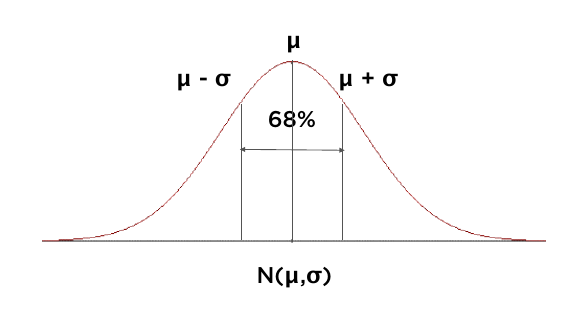
\includegraphics[trim={0 1cm 0 0}, clip, scale=0.4]{eda/nd7.png}
	\end{figure}
	
	\centering
	68\% within 1 standard deviation of mean
	
\end{frame}

\begin{frame}[t]{The Empirical Rule--3}
	
	\begin{figure} [ht]
		\centering
		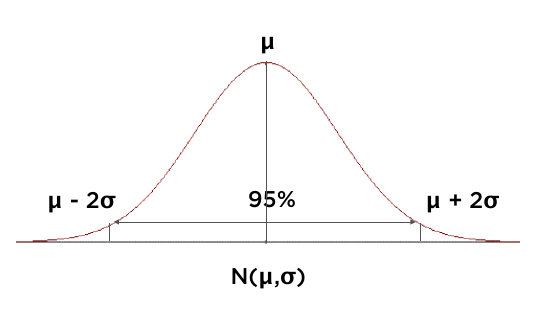
\includegraphics[trim={0 1cm 0 0}, clip, scale=0.4]{eda/nd8.png}
	\end{figure}
	
	\centering
	95\% within 2 standard deviations of mean
	
\end{frame}


\begin{frame}[t]{The Empirical Rule--4}
	
	\begin{figure} [ht]
		\centering
		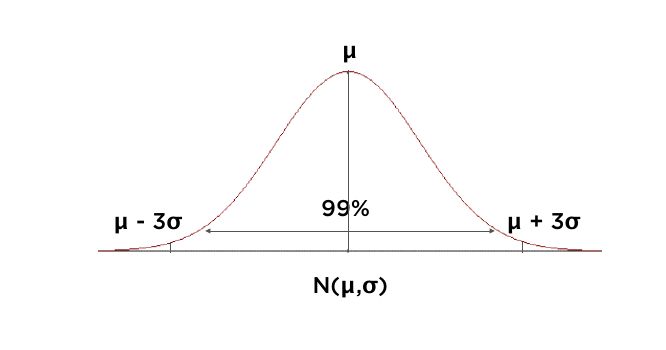
\includegraphics[trim={0 1cm 0 0}, clip, scale=0.4]{eda/nd9.png}
	\end{figure}
	
	\centering
	99\% within 3 standard deviations of mean
	
\end{frame}

\begin{frame}[t]{Impact of Outliers}
	
	\begin{figure} [ht]
		\centering
		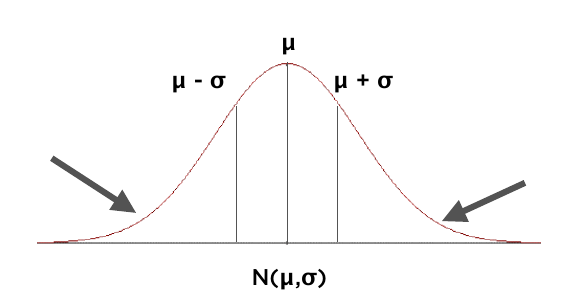
\includegraphics[trim={0 1cm 0 0}, clip, scale=0.4]{eda/nd6.png}
	\end{figure}
	
	\centering
	There will be few extreme values - the
	number of extreme values at either side of
	the mean will be the same.
\end{frame}

% Slide-n
\begin{frame}[t]{Properties of a Normal Distribution}
	\begin{itemize}
		\item The mean, mode and median are all equal.
		\item The curve is symmetric at the center (i.e. around the mean, 
		$\mu$).
		\item Exactly half of the values are to the left of center and exactly 
		half the values are to the right.
		\item The total area under the curve is 1.
	\end{itemize}

\begin{figure} [ht]
	\centering
	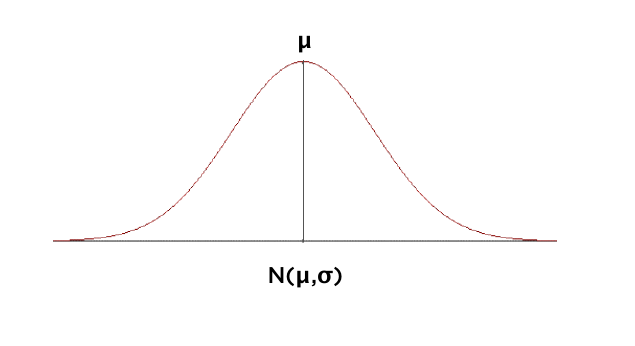
\includegraphics[trim={0 1cm 0 0}, clip, scale=0.4]{eda/nd3.png}
\end{figure}
\end{frame}

% Slide-n
\begin{frame}[t]{Role of Sigma($\sigma$)}
	\begin{figure}[h]
		\centering
		\begin{subfigure}{0.45\textwidth}
			\centering
			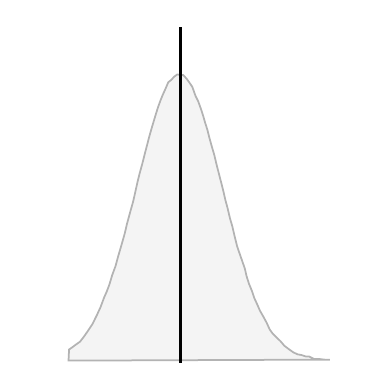
\includegraphics[scale=0.5]{eda/std1.png}
			\caption{Small Standard Deviation($\sigma$)}
			Few points far from the mean
		\end{subfigure}
		\hfil
		\begin{subfigure}{0.45\textwidth}
			\centering
			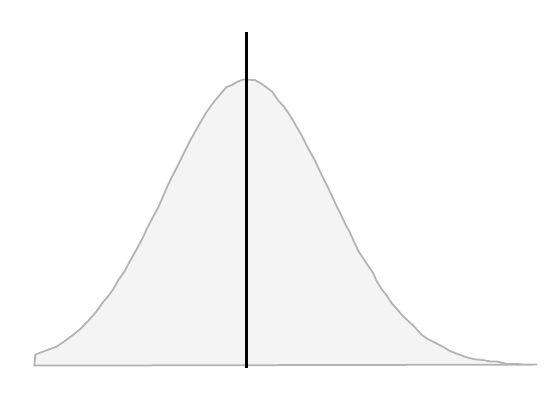
\includegraphics[scale=0.5]{eda/std2.png}
			\caption{ Large Standard Deviation($\sigma$)}
			 Many points far from the mean
			
		\end{subfigure}
		
	\end{figure}
\end{frame}
% Slide-n
\begin{frame}[t]{Z-Scores}
	\begin{itemize}
		\item Z-Scores are standardized values that can be used to compare 
		scores in different distributions.
		\item Simply put, a z-score (also called a standard score) gives you an 
		idea of how far from the mean a data point is. But more technically 
		it’s a measure of how many standard deviations below or above the 
		population mean a raw score is.
		\item A z-score can be placed on a normal distribution curve. Z-scores 
		range from -3 standard deviations (which would fall to the far left of 
		the normal distribution curve) up to +3 standard deviations (which 
		would fall to the far right of the normal distribution curve). 
		\item In order 
		to use a z-score, you need to know the population mean $\mu$ and also 
		the 
		population standard deviation $\sigma$.
	\end{itemize}

\end{frame}

% Slide-n
\begin{frame}[t]{Calculating Z-Score}
	$$
	Z = \frac{\overline{x}-\mu}{\sigma}
	$$
	
	\begin{itemize}
		\item $\overline{x}$ $\rightarrow$ mean 
		\item $\mu$ $\rightarrow$ population mean 
		\item $\sigma$ $\rightarrow$ population standard deviation
	\end{itemize}
\end{frame}


% Slide-n
\begin{frame}[t]{Calculating Z-Score}
	For example, let’s say you have a test score of 190. The test has a mean 
	($\mu$) of 150 and a standard deviation ($\sigma$) of 25. Assuming a normal 
	distribution, your z score would be
	
\end{frame}


% Slide-n
\begin{frame}[t]{Skewness--1}
	\begin{itemize}
		\item A measure of asymmetry around the mean.
		\item If one tail is longer than another, the distribution is skewed.
		\item These distributions are sometimes called asymmetric or 
		asymmetrical distributions as they don’t show any kind of symmetry.
		\item Symmetry means that one half of the distribution is a mirror 
		image of the other half.
	\end{itemize}
\begin{figure} [ht]
	\centering
	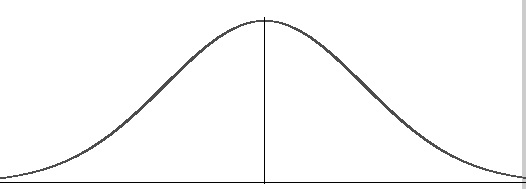
\includegraphics[trim={0 0 0.1cm 0}, clip, 
	scale=0.5]{eda/normal-distribution-probability.jpg}
	\source{https://www.statisticshowto.com/probability-and-statistics/}
\end{figure}
\end{frame}

\begin{frame}[t]{Skewness--2}
	\begin{itemize}
		\item Normally distributed data: skewness = 0
		\item Extreme values are equally likely on both
		sides of the mean.
		\item Symmetry about the mean
	\end{itemize}
\begin{figure} [ht]
	\centering
	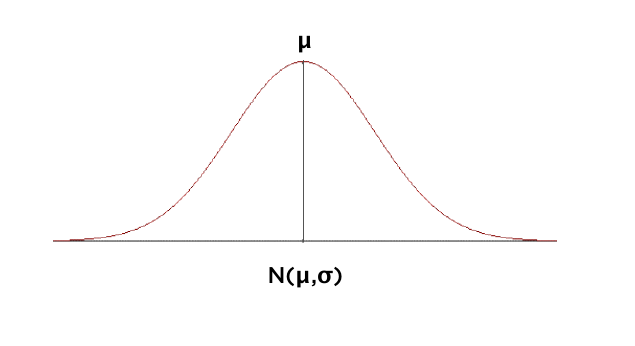
\includegraphics[trim={0 1cm 0 0}, clip, scale=0.4]{eda/nd3.png}
\end{figure}
\end{frame}
% Slide-n
\begin{frame}[t]{Negative Skewness}
	\begin{itemize}
		\item A left-skewed distribution has a long left tail.
		\item Left-skewed distributions are also called negatively-skewed 
		distributions.
		\item That’s because there is a long tail in the negative direction on 
		the number line. The mean is also to the left of the peak.
	\end{itemize}

\begin{figure} [ht]
	\centering
	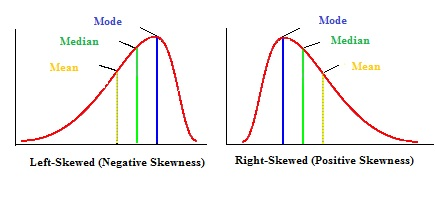
\includegraphics[trim={0 0 6cm 0}, clip, 
	scale=0.7]{eda/pearson-mode-skewness.jpg}
	\source{\url{https://www.statisticshowto.com/probability-and-statistics/}}
\end{figure}
\end{frame}

\begin{frame}[t]{Positive Skewness}
	\begin{itemize}
		\item A right-skewed distribution has a long right tail. 
		\item Right-skewed distributions are also called positive-skew 
		distributions.
		\item That’s because there is a long tail in the positive direction on 
		the number line. The mean is also to the right of the peak.
	\end{itemize}
	
	\begin{figure} [ht]
		\centering
		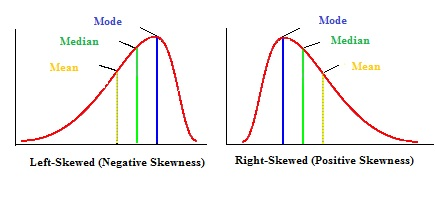
\includegraphics[trim={6cm 0 0 0}, clip, 
		scale=0.7]{eda/pearson-mode-skewness.jpg}
		\source{\url{https://www.statisticshowto.com/probability-and-statistics/}}
	\end{figure}
\end{frame}


% Slide-n
\begin{frame}[t]{Mean and Median in Skewed Distributions}
	In a normal distribution, the mean and the median are the same 
	number while the mean and median in a skewed distribution become 
	different numbers.
	\begin{itemize}
		\item A left-skewed, negative distribution will have the mean to the 
		left of the median.
	\end{itemize}
	\begin{figure} [ht]
		\centering
		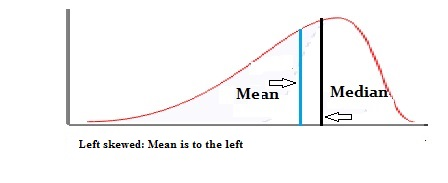
\includegraphics[width=0.6\textwidth]{eda/left-skewed.jpg}
		\source{\url{https://www.statisticshowto.com/probability-and-statistics/}}
	\end{figure}
\end{frame}

% Slide-n
\begin{frame}[t]{Mean and Median in Skewed Distributions}
	\begin{itemize}
		\item A right-skewed, negative distribution will have the mean to the 
		right of the median.
	\end{itemize}
	\begin{figure} [ht]
		\centering
		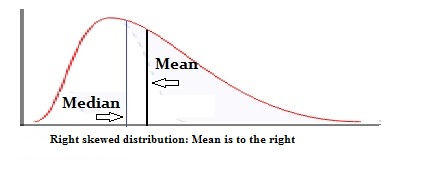
\includegraphics[width=0.6\textwidth]{eda/right-skewed.jpg}
		\source{\url{https://www.statisticshowto.com/probability-and-statistics/}}
	\end{figure}
\end{frame}

% Slide-n
\begin{frame}[t]{Kurtosis}
Kurtosis is a statistical measure that defines how heavily the tails of a 
distribution differ from the tails of a normal distribution. In other words, 
kurtosis identifies whether the tails of a given distribution contain extreme 
values.
\end{frame}
% Slide-n
\begin{frame}[t]{Kurtosis}
	\begin{itemize}
		\item Normally distributed data: kurtosis = 3
		\item Excess kurtosis = kurtosis - 3
		\item Kurtosis ~ Tail risk
		\item High kurtosis => extreme events more
		likely than in normal distribution.
	\end{itemize}
\end{frame}


